\documentclass[a4paper,14pt]{extreport}
\usepackage[left=1.5cm,right=1.5cm,
    top=1.5cm,bottom=2cm,bindingoffset=0cm]{geometry}
\usepackage{scrextend}
\usepackage[T1,T2A]{fontenc}
\usepackage[utf8]{inputenc}
\usepackage[english,russian,ukrainian]{babel}
\usepackage{tabularx}
\usepackage{amssymb}
\usepackage{color}
\usepackage{amsmath}
\usepackage{mathrsfs}
\usepackage{listings}
\usepackage{graphicx}
\graphicspath{ {./images/} }
\usepackage{lipsum}
\usepackage{xcolor}
\usepackage{hyperref}
\usepackage{tcolorbox}
\usepackage{tikz}
\usepackage[framemethod=TikZ]{mdframed}
\usepackage{wrapfig,boxedminipage,lipsum}
\mdfdefinestyle{MyFrame}{%
linecolor=blue,outerlinewidth=2pt,roundcorner=20pt,innertopmargin=\baselineskip,innerbottommargin=\baselineskip,innerrightmargin=20pt,innerleftmargin=20pt,backgroundcolor=gray!50!white}
 \usepackage{csvsimple}
 \usepackage{supertabular}
\usepackage{pdflscape}
\usepackage{fancyvrb}
%\usepackage{comment}
\definecolor{ggreen}{rgb}{0.4,1,0}
\definecolor{rred}{rgb}{1,0.1,0.1}
\definecolor{aquamarine}{rgb}{0.5, 1.0, 0.83}
\definecolor{amber}{rgb}{1.0, 0.75, 0.0}
\definecolor{babyblue}{rgb}{0.54, 0.81, 0.94}
\usepackage{array,tabularx}
\usepackage{colortbl}

\usepackage{varwidth}
\tcbuselibrary{skins}
\usepackage{fancybox}

\usetikzlibrary{calc}
\makeatletter
\newlength{\mylength}
\xdef\CircleFactor{1.1}
\setlength\mylength{\dimexpr\f@size pt}
\newsavebox{\mybox}
\newcommand*\circled[2][draw=blue]{\savebox\mybox{\vbox{\vphantom{WL1/}#1}}\setlength\mylength{\dimexpr\CircleFactor\dimexpr\ht\mybox+\dp\mybox\relax\relax}\tikzset{mystyle/.style={circle,#1,minimum height={\mylength}}}
\tikz[baseline=(char.base)]
\node[mystyle] (char) {#2};}
\makeatother




\usepackage{float}
\usepackage{wrapfig}
\usepackage{framed}
%for nice Code{
\lstdefinestyle{customc}{
  belowcaptionskip=1\baselineskip,
  breaklines=true,
  frame=L,
  xleftmargin=\parindent,
  language=C,
  showstringspaces=false,
  basicstyle=\small\ttfamily,
  keywordstyle=\bfseries\color{green!40!black},
  commentstyle=\itshape\color{purple!40!black},
  identifierstyle=\color{blue},
  stringstyle=\color{orange},
}
\lstset{escapechar=@,style=customc}
%}


\begin{document}
\pagecolor{white}
\begin{titlepage}
  \begin{center}
    \large
    Національний технічний університет України \\ "Київський політехнічний інститут імені Ігоря Сікорського"


    Факультет Електроніки

    Кафедра мікроелектроніки
    \vfill

    \textsc{ЗВІТ}\\

    {\Large Про виконання лабораторної роботи №1\\
      з дисципліни: «Вакуумна та плазмова електроніка»\\[1cm]

        ДОСЛІДЖЕННЯ ФОТОЕФЕКТУ


    }
  \bigskip
\end{center}
\vfill

\newlength{\ML}
\settowidth{\ML}{«\underline{\hspace{0.4cm}}» \underline{\hspace{2cm}}}
\hfill
\begin{minipage}{1\textwidth}
Виконавець:\\
Студент 3-го курсу \hspace{4cm} $\underset{\text{(підпис)}}{\underline{\hspace{0.2\textwidth}}}$  \hspace{1cm}Б.\,В.~Лищенко\\
\vspace{1cm}

Перевірив: \hspace{5.9cm} $\underset{\text{(підпис)}}{\underline{\hspace{0.2\textwidth}}}$  \hspace{1cm}О.\,М.~Бевза\\

\end{minipage}

\vfill

\begin{center}
2021
\end{center}
\end{titlepage}



\textbf{Мета роботи}: Дослідження вольт-амперних і світлових характеристик фотоелементів для
видимого спектру світла.
\begin{center}\textbf{Завдання}\end{center}\par
\newtcbox{\xmybox}[1][red]{on line, arc=7pt,colback=#1!10!white,colframe=#1!50!black, before upper={\rule[-3pt]{0pt}{10pt}},boxrule=1pt, boxsep=0pt,left=6pt,right=6pt,top=2pt,bottom=2pt}

1 Зняти ВАХ для 4-х значень довжин хвиль вибравши з набору: \underline{200} нм, \underline{400} нм, 440 нм, 470
нм, 520 нм, 580 нм, 610 нм, \underline{650} нм, \underline{700} нм, 750 нм на вибір при інтенсивності 50\% та 100\%. Побудувати окремо два сімейства кривих для 50\% та 100\% інтенсивності для 3-х різних матеріалів мішені (на вибір). Значення для графіків брати з показань у вікнах «Напруга зміщення» та «Струм».\\

2 Зняти світлові характеристики. Побудувати сімейство кривих залежності
Струм(інтенсивність світла) для довжин хвиль 200 нм, 400 нм, 440 нм для мішені з натрія (або іншого матеріалу фотомішені на вибір). Значення для графіків брати з показань у вікнах «Струм» та «Інтенсивність».\\

3 Побудувати сімейство кривих залежності Енергія(частота) при будь-якій інтенсивності при \underline{50\%} на
всьому інтервалі частот для матеріалів мішені: натрій, цинк, мідь, платина, кальцій, магній.\\

\vspace{1cm}

\begin{center}1\end{center}
\begin{figure}[h]
\center{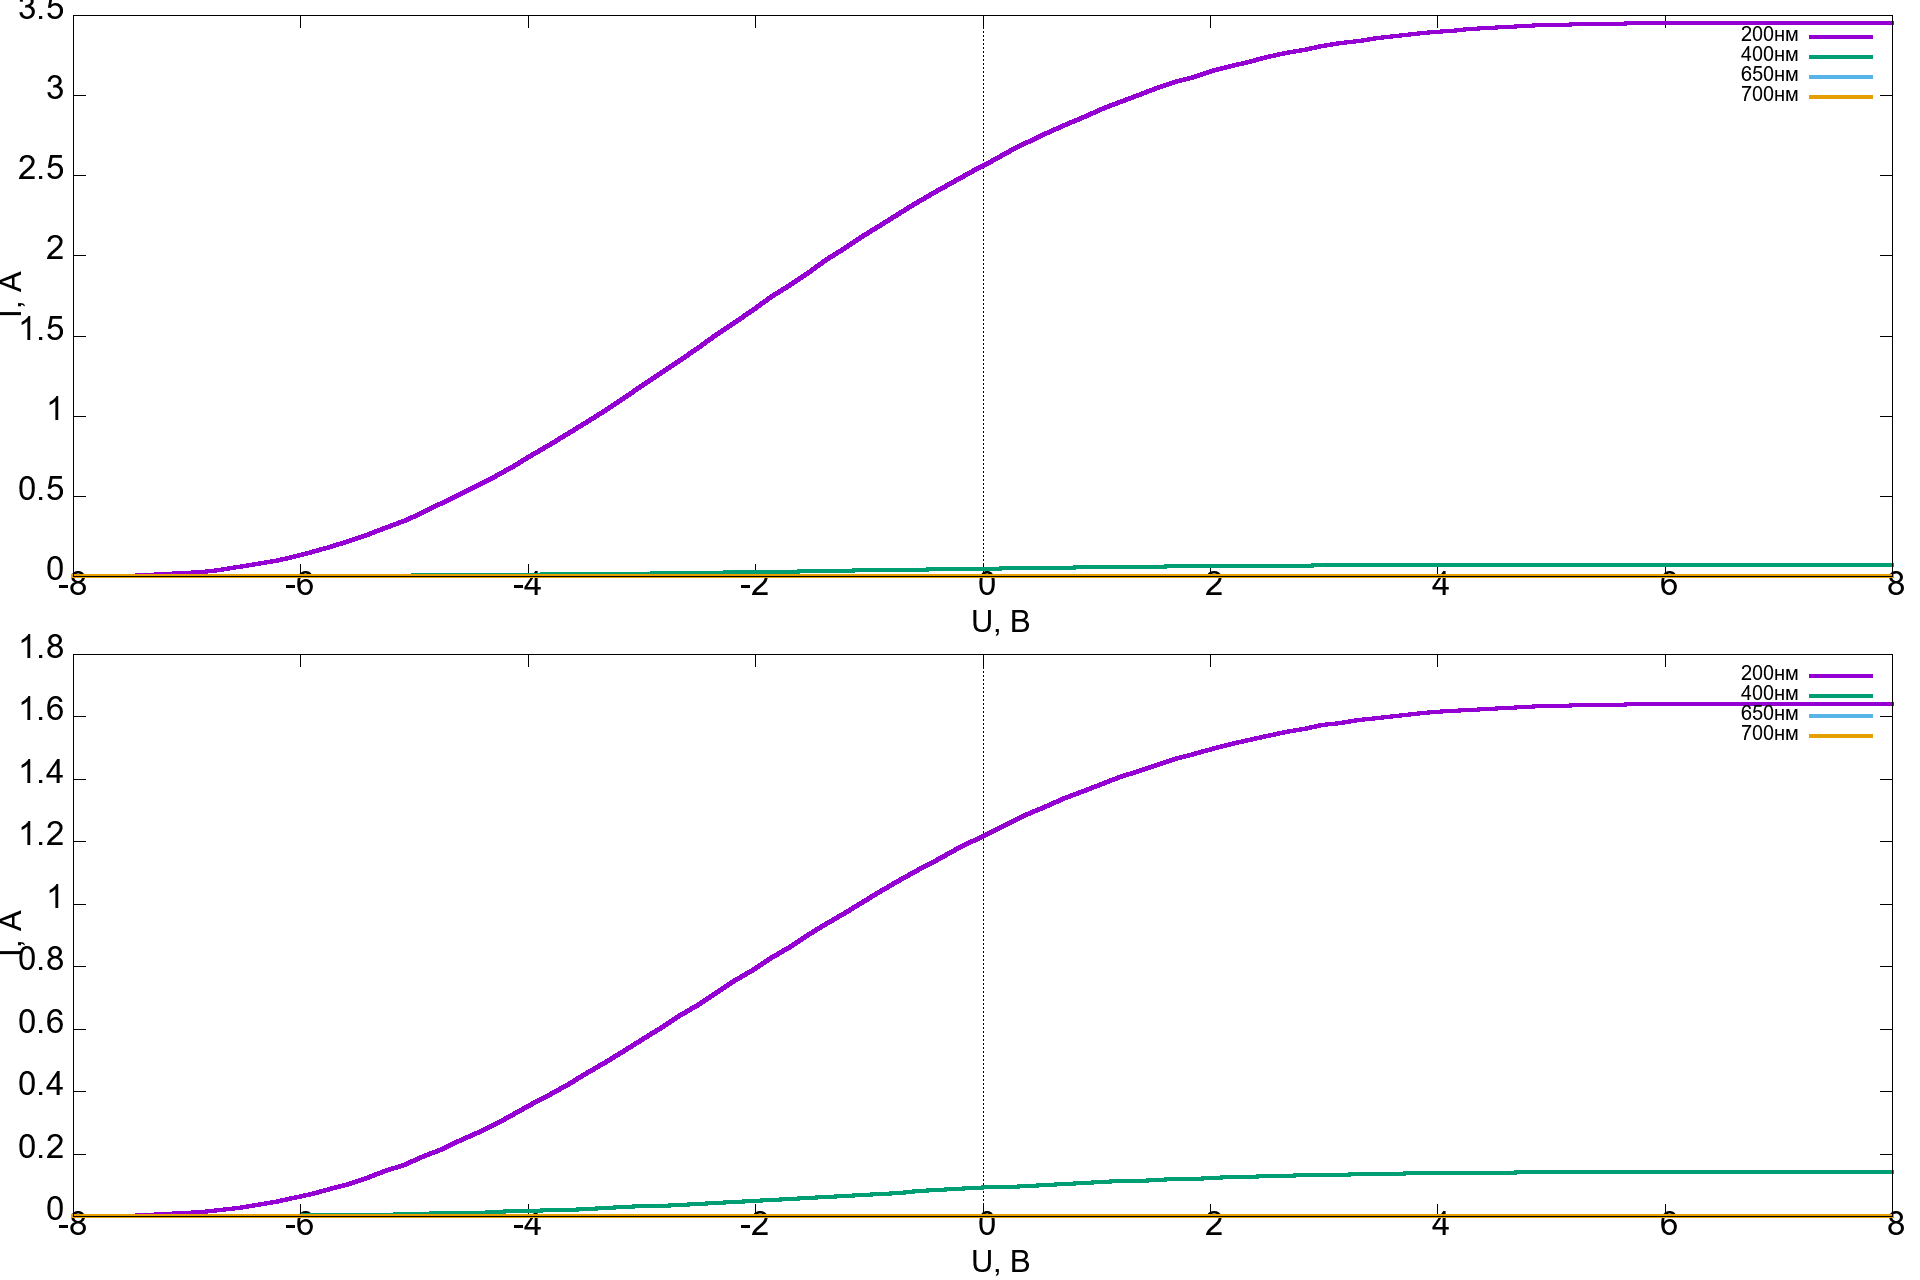
\includegraphics[width=0.8\linewidth]{50-100_Na.png}}
\caption{Сiмейства кривих для 50\% та 100\% iнтенсивностi для Натрію.}
\label{ris1}
\end{figure}

\begin{figure}[h]
\center{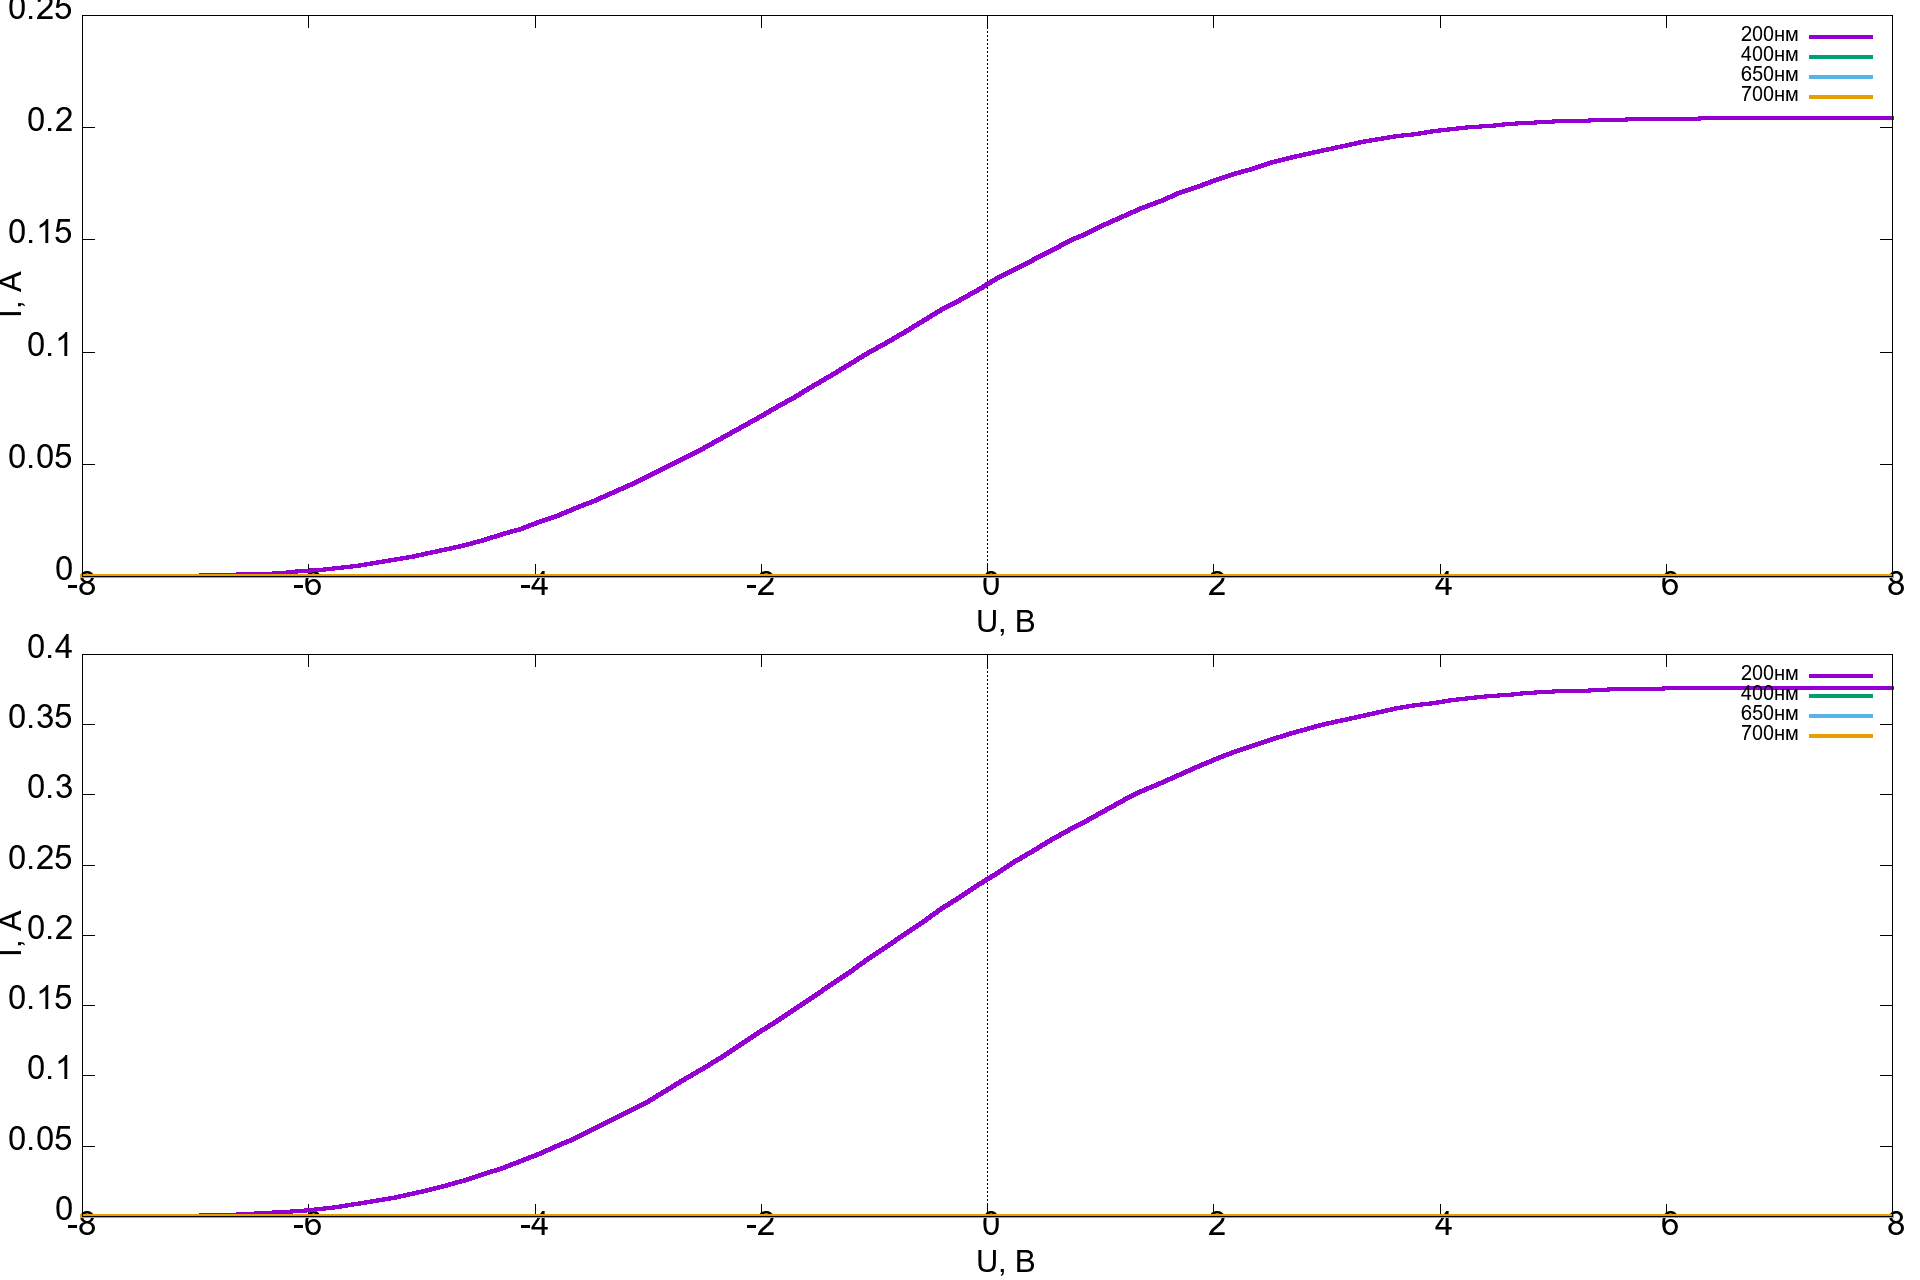
\includegraphics[width=0.8\linewidth]{50-100_Zn.png}}
\caption{Сiмейства кривих для 50\% та 100\% iнтенсивностi для Цинку.}
\label{ris1}
\end{figure}


\begin{figure}[h]
\center{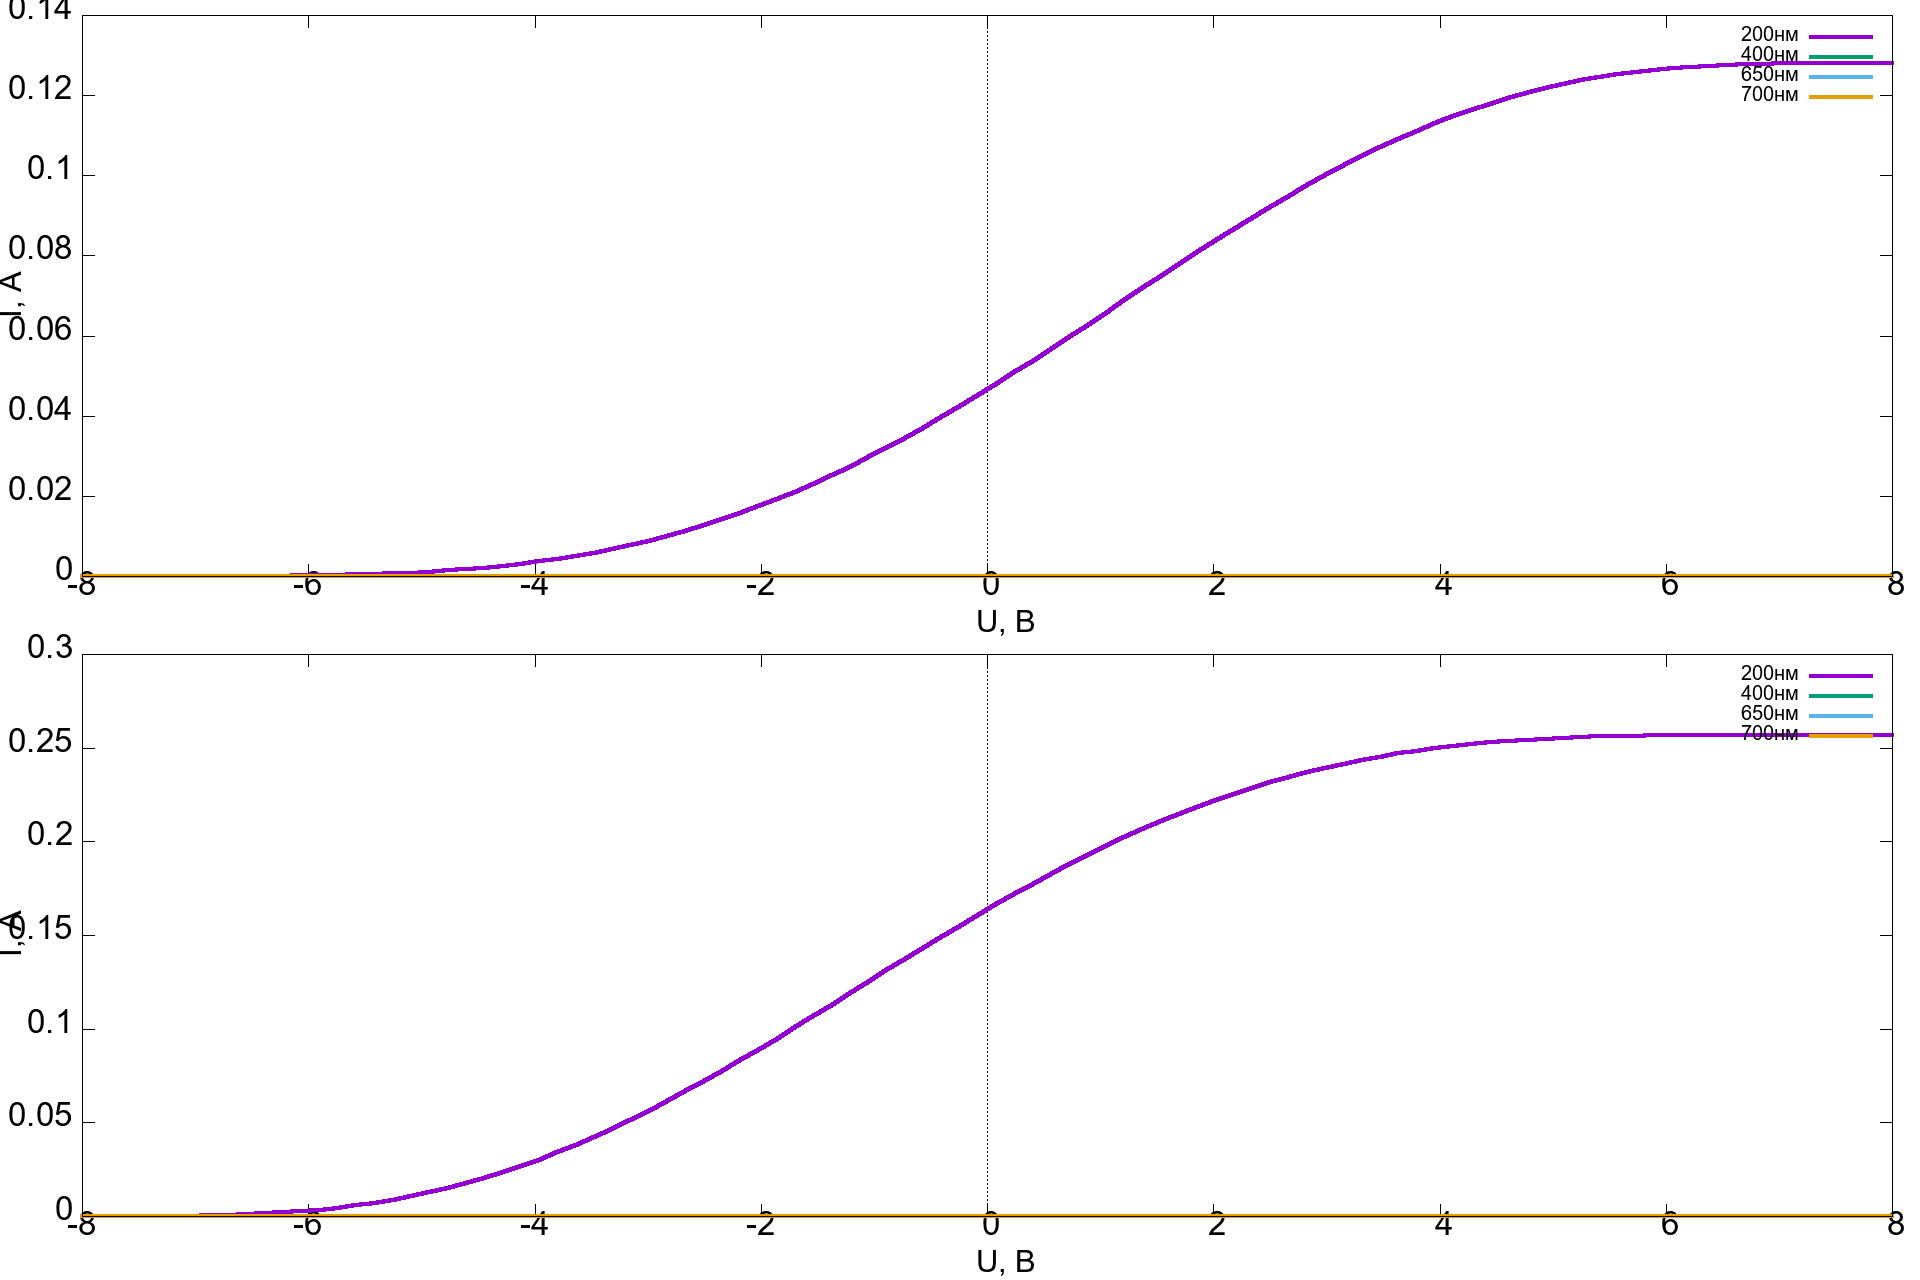
\includegraphics[width=0.8\linewidth]{50-100_Cu.png}}
\caption{Сiмейства кривих для 50\% та 100\% iнтенсивностi для Міді.}
\label{ris1}
\end{figure}





% #######################################
%###                2                ###
%######################################
\clearpage
\newpage
\begin{center}2\end{center}

\begin{figure}[h]
\center{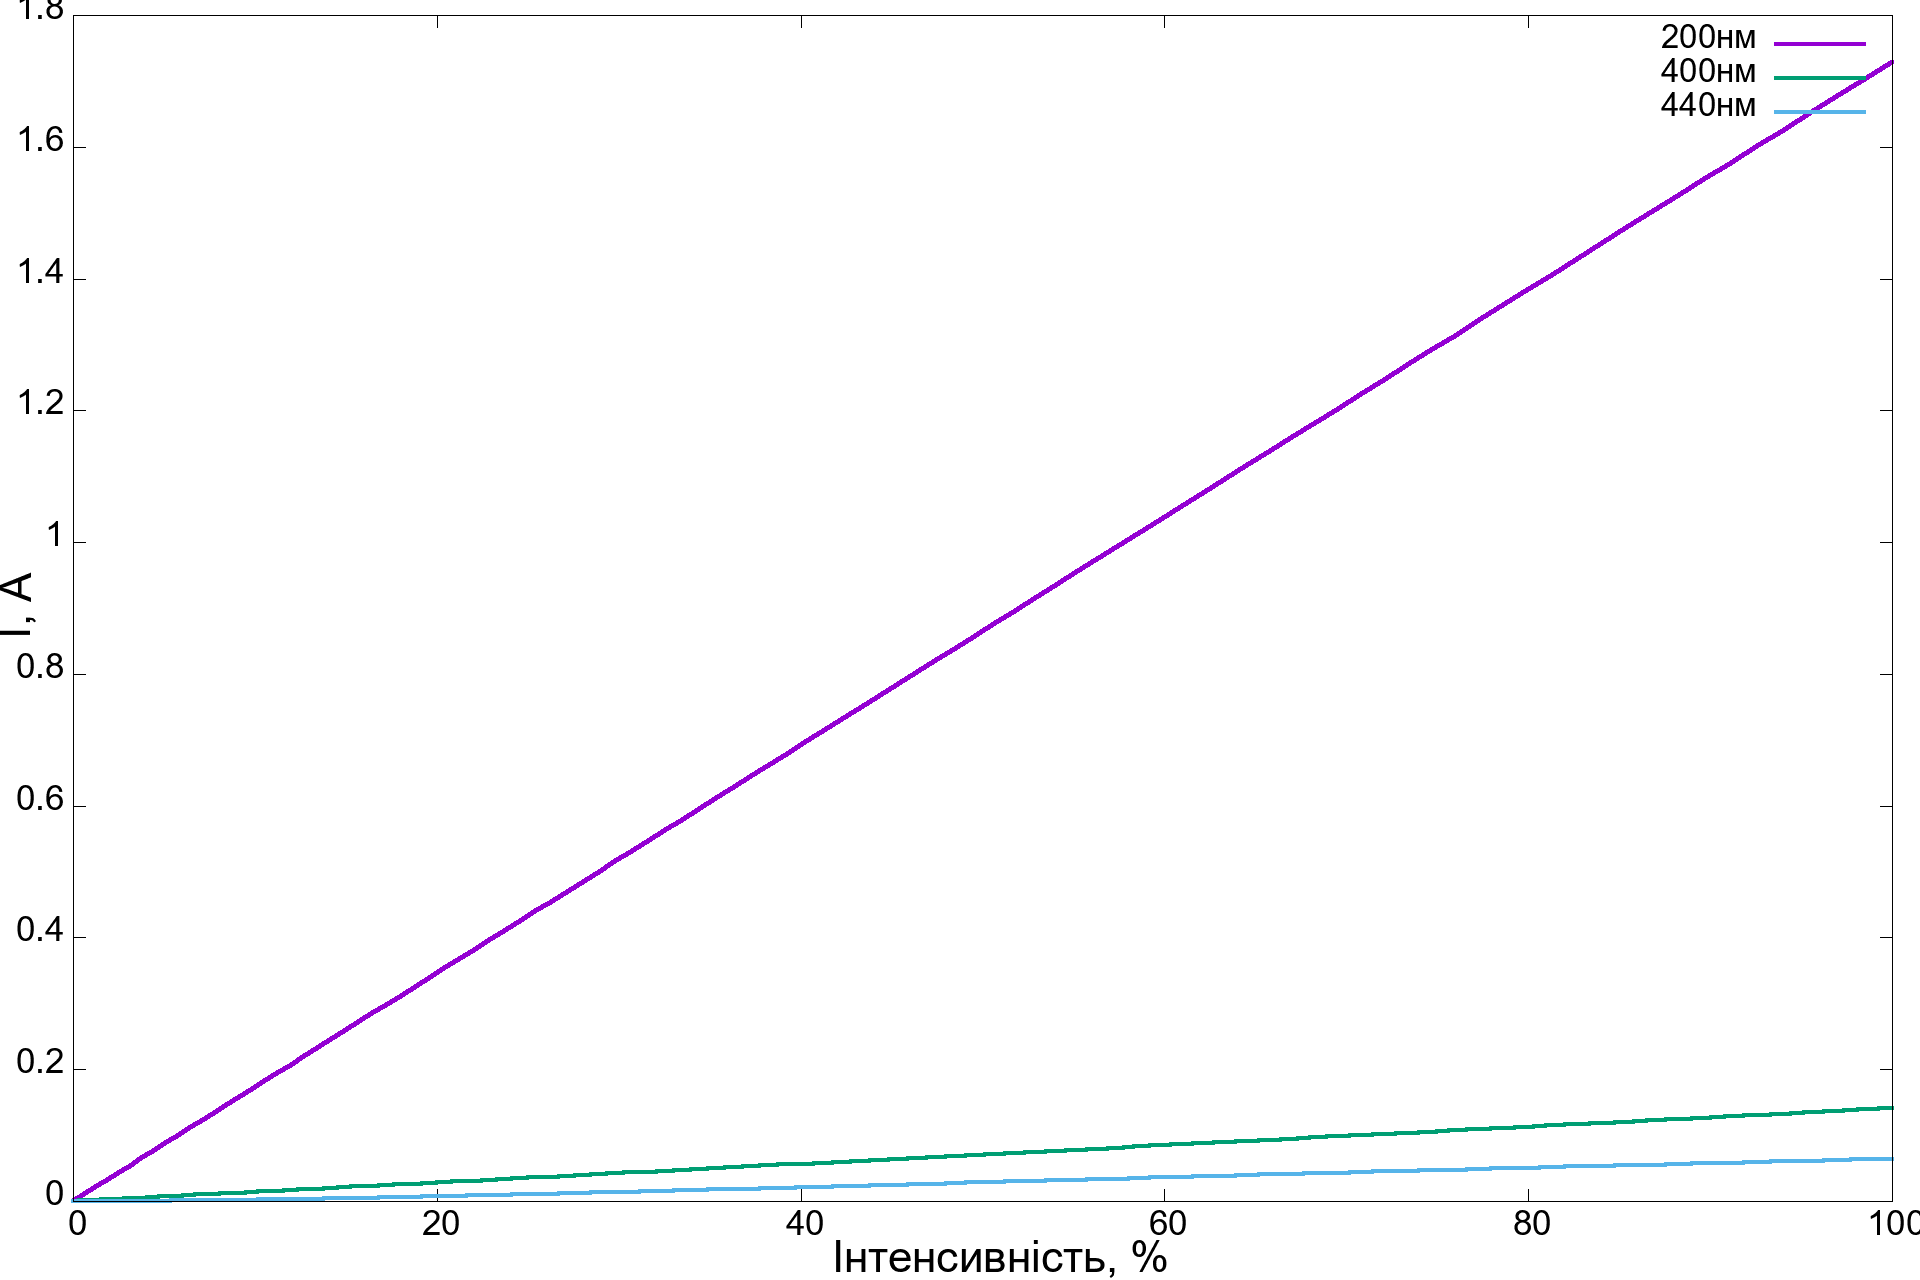
\includegraphics[width=0.9\linewidth]{2Na.png}}
\caption{сiмейство кривих залежностi Струм(iнтенсивнiсть свiтла) для довжин хвиль 200 нм, 400 нм, 440 нм для мiшенi з натрiя.}
\label{ris7}
\end{figure}


\begin{center}3\end{center}
\begin{figure}[h]
\center{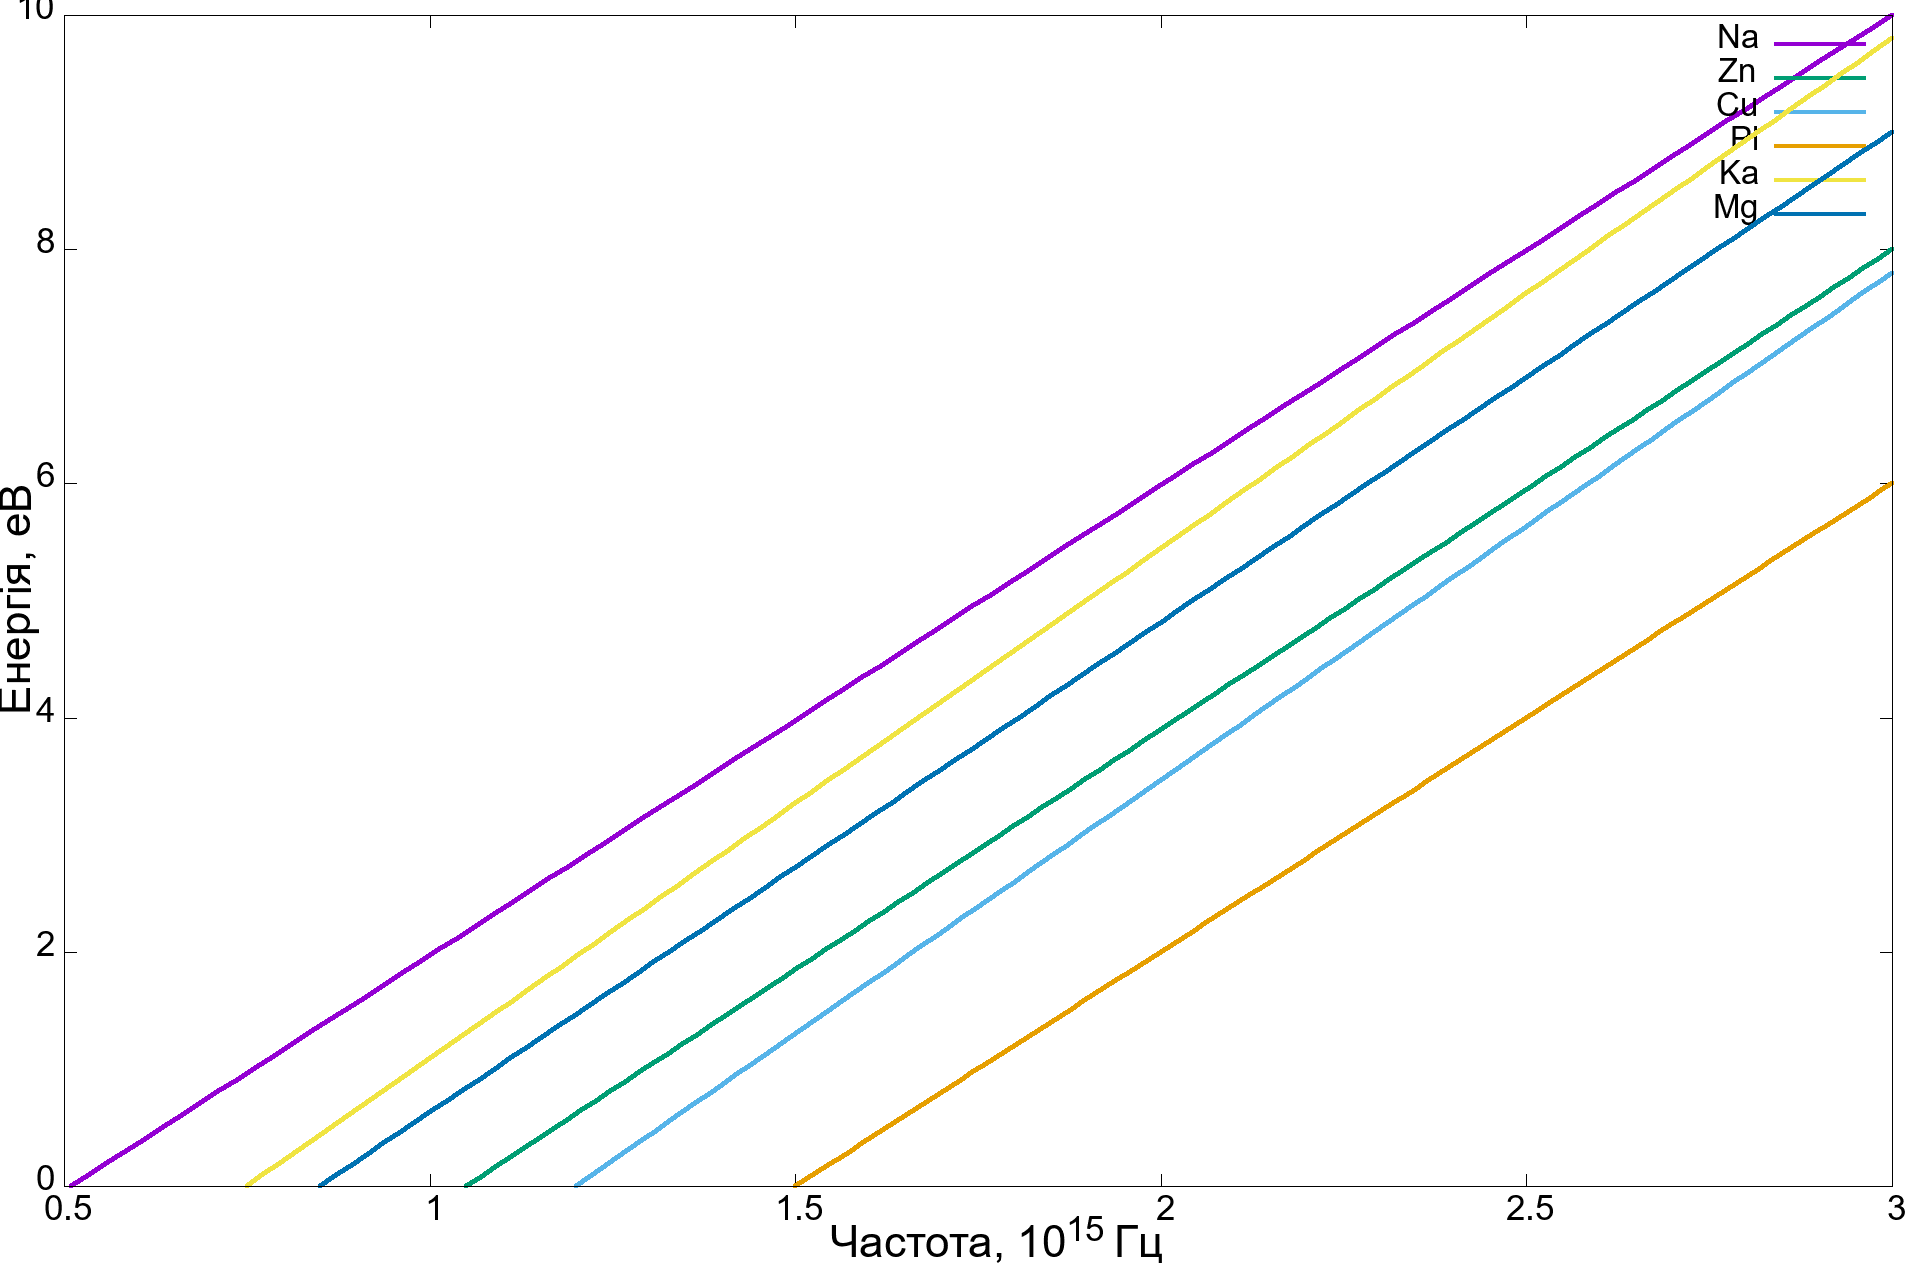
\includegraphics[width=0.9\linewidth]{3part.png}}
\caption{Ciмейство кривих залежностi Енергiя(частота) при iнтенсивностi 50\% на всьому iнтервалi частот для натрiй, цинк, мiдь, платина, кальцiй і магнiй.}
\label{ris8}
\end{figure}
\newpage
Висновок:\\
в данiй лабораторнiй роботi можна наочно переконається в iснуваннi внутрiшнього фотоефекта. При порiвняннi ВАХ металiв фотомiшенi, можна зазначити, що найбiльше значення фотоструму має натрій, тобто, при інтенсивності 100\% струм насичення буде приблизно 1.65 А, а найменше значення має мiдь, при інтенсивності 100\% струм насичення дорівнює приблизно 0.26 А. А от чутлiвiсть яка є основним параметром фотоелемента, яка дуже добре спостерiгається в материалi на короткiй довжинi хвилi. Також добре помiтно, що кожен матерiал має своє граничне значення частоти та довжина хвилi свiтла, вiд яких залежить вiдбуватиметься фотоефект чи нi, дивлячись на графіки залежності енергії від частоти, можна замітити, що для натрію це буде $0,5\cdot10^{15}$ Гц, а для міді це значення $1,2\cdot10^{15}$ Гц . За допомогою останнього сiмейства можна зробити висновок, що при збiльшеннi частоти свiтла, енергiя яку набувають електрони буде поступово збiльшуватись. Також беручи до уваги те що вийшло на останньому рисунку можна визначити роботу виходу яка безпосередньо впливає на величину самого фотоструму. Виходячи з того, що чим бiльше робота виходу, тим менше енергiя електрона тому виходить, що в данному випадку найбiльше значення роботи виходу має платина, i вже далi мiдь, цинк, магнiй, кальцiй та натрiй.

\end{document}
